\chapter{物理世界模型：从约束优化到智能本质}

 

\vspace{1cm}

\begin{center}
\textit{"如果说拉格朗日力学描述了死物的运动规律，\\
那么我们如何用同样的数学语言描述智能体的思考与行动？"}
\end{center}

\vspace{1cm}

 

% ====================================================================================

\section*{引言：约束优化的终极问题}

% ====================================================================================

 

\marginnote{这一章是全书的Grand Finale。我们将看到，从牛顿力学到深度学习，从机器人控制到世界模型，所有这些看似不同的领域，都可以用同一个数学语言来统一：\textbf{约束优化}。}

 

让我们回顾这本书的旅程：

 

\begin{itemize}

    \item 第一章，我们从$F = ma$出发，看到拉格朗日如何用\textbf{约束优化}重新表述力学

    \item 中间的章节，我们学习了如何用神经网络求解PDE（PINN）、学习算子（神经算子）、处理多智能体博弈

    \item 现在，站在全书的终点，我们要问一个更深刻的问题：

\end{itemize}

 

\begin{quote}

\textbf{智能的本质是什么？}

\end{quote}

 

一块石头从山上滚下，遵循最小作用量原理——它"知道"如何找到最省能量的路径。但石头不是智能的。

 

一只猫追逐老鼠，也在某种意义上"优化"——但它的目标函数是什么？它的约束是什么？

 

一个自动驾驶系统在复杂的城市环境中导航，既要到达目的地（优化），又不能撞人（约束），还要预测其他车辆的行为（建模）。

 

\begin{framed}

\textbf{本章核心问题}：

 

如何用我们学过的数学工具——约束优化、动力系统、神经网络——来理解和构建\textbf{能够感知、预测、规划、行动}的智能系统？

 

\textbf{本章结构}：

\begin{enumerate}

    \item 什么是世界模型？——从"拟合数据"到"理解结构"

    \item 具身智能的数学本质——物理约束下的安全控制

    \item 可微物理——当牛顿定律变成计算图

    \item 终极猜想——自由能原理与智能的统一理论

\end{enumerate}

\end{framed}

 

% ====================================================================================

\section{什么是世界模型？}

% ====================================================================================

 

\subsection{从模型说起：什么是"理解"？}

 

在物理学中，"模型"是对现实世界的数学抽象。牛顿力学是一个模型，麦克斯韦方程是一个模型，薛定谔方程也是一个模型。

 

\begin{example}[你已经见过很多"模型"]

\begin{itemize}

    \item \textbf{单摆模型}：用角度$\theta$和角速度$\dot{\theta}$描述摆的状态

    \item \textbf{弹簧模型}：$F = -kx$，用位移描述弹力

    \item \textbf{热传导模型}：$\frac{\partial T}{\partial t} = \alpha \nabla^2 T$，用温度场描述热量流动

\end{itemize}

这些模型的共同点是：\textbf{用少数变量捕捉系统的本质行为}。

\end{example}

 

\begin{definition}[世界模型的直观定义]

在人工智能中，\textbf{世界模型}（World Model）是智能体对环境的内部表示。简单来说：

 

\begin{center}

\fbox{\textbf{世界模型 = 智能体脑中的"物理模拟器"}}

\end{center}

 

它回答一个核心问题：\textbf{如果我做了动作$a$，世界会变成什么样？}

\end{definition}

 

用数学语言表述：给定当前状态$s_t$和动作$a_t$，世界模型预测下一个状态$s_{t+1}$：

\begin{equation}
    \boxed{s_{t+1} = f(s_t, a_t) + \epsilon}
\end{equation}

其中：

\begin{itemize}

    \item $s_t$：\textbf{当前状态}——可以是机器人的位置、速度，也可以是游戏画面

    \item $a_t$：\textbf{动作}——智能体采取的行动，如"向左转"、"加速"

    \item $f$：\textbf{动力学函数}——描述状态如何演化的规则

    \item $\epsilon$：\textbf{不确定性}——世界并非完全可预测

\end{itemize}

 

\begin{example}[世界模型的生活实例]

想象你在打台球：

\begin{itemize}

    \item \textbf{状态}$s_t$：所有球的位置

    \item \textbf{动作}$a_t$：你击球的力度和角度

    \item \textbf{世界模型}$f$：预测击球后所有球会滚到哪里

\end{itemize}

 

一个台球高手脑中有一个精确的"物理模拟器"——他能在击球前"想象"出球的运动轨迹。这就是世界模型的本质！

\end{example}

 

\subsection{两种范式之争：像素vs本质}

 

当前AI领域对"世界模型"有两种截然不同的哲学。这场争论的核心是：\textbf{我们应该在什么空间中建模？}

 

\subsubsection{生成式世界模型（OpenAI/Sora路线）}

 

\marginnote{Sora是OpenAI在2024年发布的视频生成模型，能够生成高度逼真的视频。它被一些人认为是"物理模拟器"，因为它似乎"理解"了物体如何运动。}

 

核心思想：\textbf{预测原始像素}。

 

如果一个模型能够准确预测视频的下一帧，那么它一定"理解"了物理规律——因为没有理解物理，就无法预测物体会怎么运动。

 

数学表述：学习条件概率分布

\begin{equation}
    P(x_{t+1} | x_1, x_2, \ldots, x_t)
\end{equation}

其中$x_t$是第$t$帧的像素（比如一张$256 \times 256$的图片有65536个像素值）。

 

\begin{example}[视频预测作为物理模拟]

想象一个视频：一个球从桌子边缘滚落。

 

要准确预测下一帧，模型需要"知道"：

\begin{itemize}

    \item 重力会让球加速下落（$a = g \approx 9.8 \text{m/s}^2$）

    \item 球是圆的，所以会滚动而不是滑动

    \item 空气阻力可以忽略（对于慢速运动）

    \item 球落地后会弹起（如果是弹性球）

\end{itemize}

 

如果模型能预测这些，是不是意味着它"学会"了物理？

\end{example}

 

\subsubsection{联合嵌入预测架构（LeCun/JEPA路线）}

 

\marginnote{\textbf{Yann LeCun}(1960--)：2018年图灵奖得主（与Hinton、Bengio共获），卷积神经网络之父，现任Meta首席AI科学家。他在1990年代开发的LeNet是现代CNN的鼻祖。近年他大力推动``世界模型''研究方向，批评纯语言模型是``通往AGI的错误道路''。}

 

Yann LeCun对生成式路线的批评是尖锐的：

 

\begin{quote}

\textit{"预测像素是在浪费算力去拟合随机噪声。风吹动树叶的每一个细节是不可预测的，但这不重要！重要的是树在那里，风在吹。"}

\end{quote}

 

核心思想：\textbf{在抽象特征空间预测，而不是在像素空间}。

 

\begin{definition}[JEPA架构——用大白话解释]

\textbf{联合嵌入预测架构}（Joint-Embedding Predictive Architecture，JEPA）的思想是：

\begin{enumerate}

    \item \textbf{先压缩}：把高维的像素压缩成低维的"本质特征"

    \item \textbf{再预测}：在特征空间做预测（而不是在像素空间）

    \item \textbf{比较特征}：预测的特征和真实的特征应该接近

\end{enumerate}

\end{definition}

 

用数学语言：

\begin{itemize}

    \item \textbf{编码器}$E$：将观测$x$（如图片）映射到抽象表征$s = E(x)$

    \item \textbf{预测器}$P$：在表征空间预测$\hat{s}_{t+1} = P(s_t, a_t)$

    \item \textbf{距离函数}$D$：衡量预测与真实表征的距离$D(\hat{s}_{t+1}, s_{t+1})$

\end{itemize}

 

\begin{figure}[htbp]

\centering

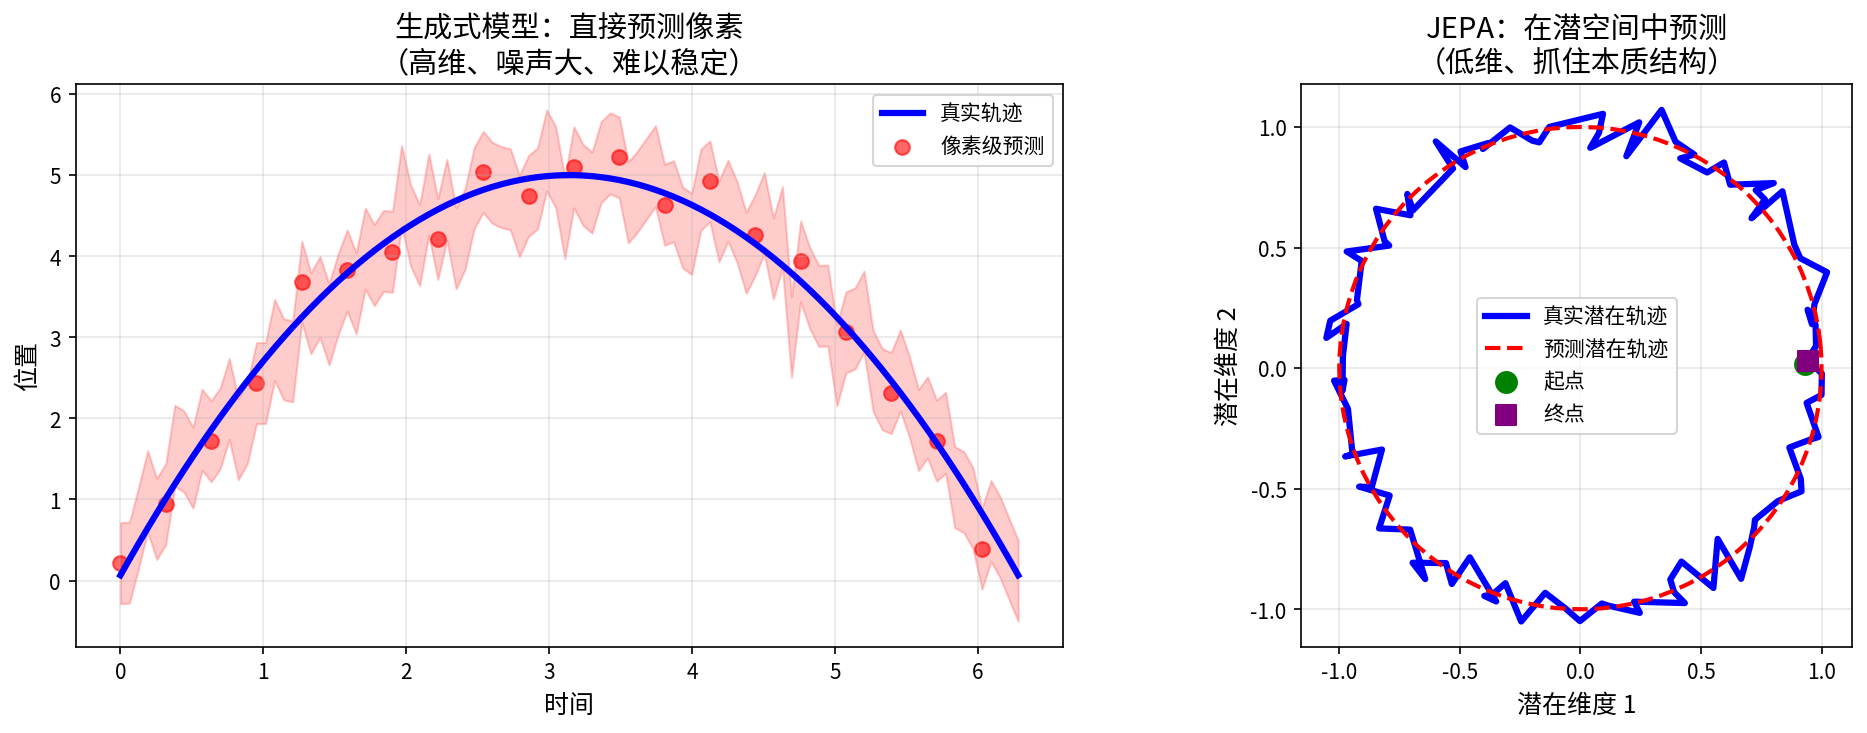
\includegraphics[width=0.95\textwidth]{figs_chap16/paradigm_comparison.png}

\caption{两种世界模型范式对比。左图：生成式模型直接预测像素，预测结果有噪声；右图：JEPA在低维潜空间预测，轨迹更加平滑、本质。}

\label{fig:paradigm_comparison}

\end{figure}

 

\begin{keyinsight}

\textbf{两种范式的约束优化视角}：

 

\textbf{生成式模型}：试图拟合整个数据分布$P(x)$

\begin{equation}
    \min_\theta \E_{x \sim \text{data}}[-\log P_\theta(x)]
\end{equation}

这是一个\textbf{无约束}的密度估计问题——要建模所有细节。

 

\textbf{JEPA}：学习表征空间中的\textbf{约束关系}

\begin{equation}
    \min_{E, P} \E[D(P(E(x_t), a_t), E(x_{t+1}))] \quad \text{s.t. 表征不能坍缩为常数}
\end{equation}

这是一个\textbf{有约束}的流形学习问题——只学习本质特征。

\end{keyinsight}

 

\begin{example}[类比：记忆 vs 理解]

想象两个学生准备考试：

\begin{itemize}

    \item \textbf{学生A}（生成式）：把课本逐字背下来，包括每个标点符号

    \item \textbf{学生B}（JEPA）：理解核心概念，用自己的话总结

\end{itemize}

学生A的"模型"可以完美复述课本，但占用大量记忆。学生B的"模型"更紧凑，而且能举一反三。

 

JEPA的哲学就是：\textbf{学习本质，忽略细节}。

\end{example}

 

\subsection{潜空间动力学：在梦境中学习}

 

无论选择哪种范式，一个共同的思想是：在\textbf{潜空间}（latent space）中建模动力学。

 

\begin{definition}[潜空间——什么是"潜"？]

"潜空间"这个名字来自"潜在变量"（latent variable）——它是隐藏在数据背后、我们无法直接观测的变量。

 

\textbf{类比}：你看到一个人在笑（观测），但你看不到他的心情（潜变量）。心情是"潜在"的，但它决定了外在表现。

\end{definition}

 

\begin{definition}[潜空间动力学模型的三个组件]

一个完整的潜空间动力学模型包含三个部分：

\begin{align}
    z_t &= \text{Encoder}(o_t) \quad \text{（\textbf{感知}：把观测压缩成潜态）} \\
    z_{t+1} &= \text{Dynamics}(z_t, a_t) \quad \text{（\textbf{预测}：潜态如何演化）} \\
    \hat{o}_{t+1} &= \text{Decoder}(z_{t+1}) \quad \text{（\textbf{想象}：从潜态还原观测）}
\end{align}

 

其中：

\begin{itemize}

    \item $o_t$：\textbf{观测}（observation），如摄像头拍到的图像，维度很高

    \item $z_t$：\textbf{潜态}（latent state），压缩后的表示，维度很低

    \item $a_t$：\textbf{动作}（action），智能体的行为

\end{itemize}

\end{definition}

 

\begin{figure}[htbp]

\centering

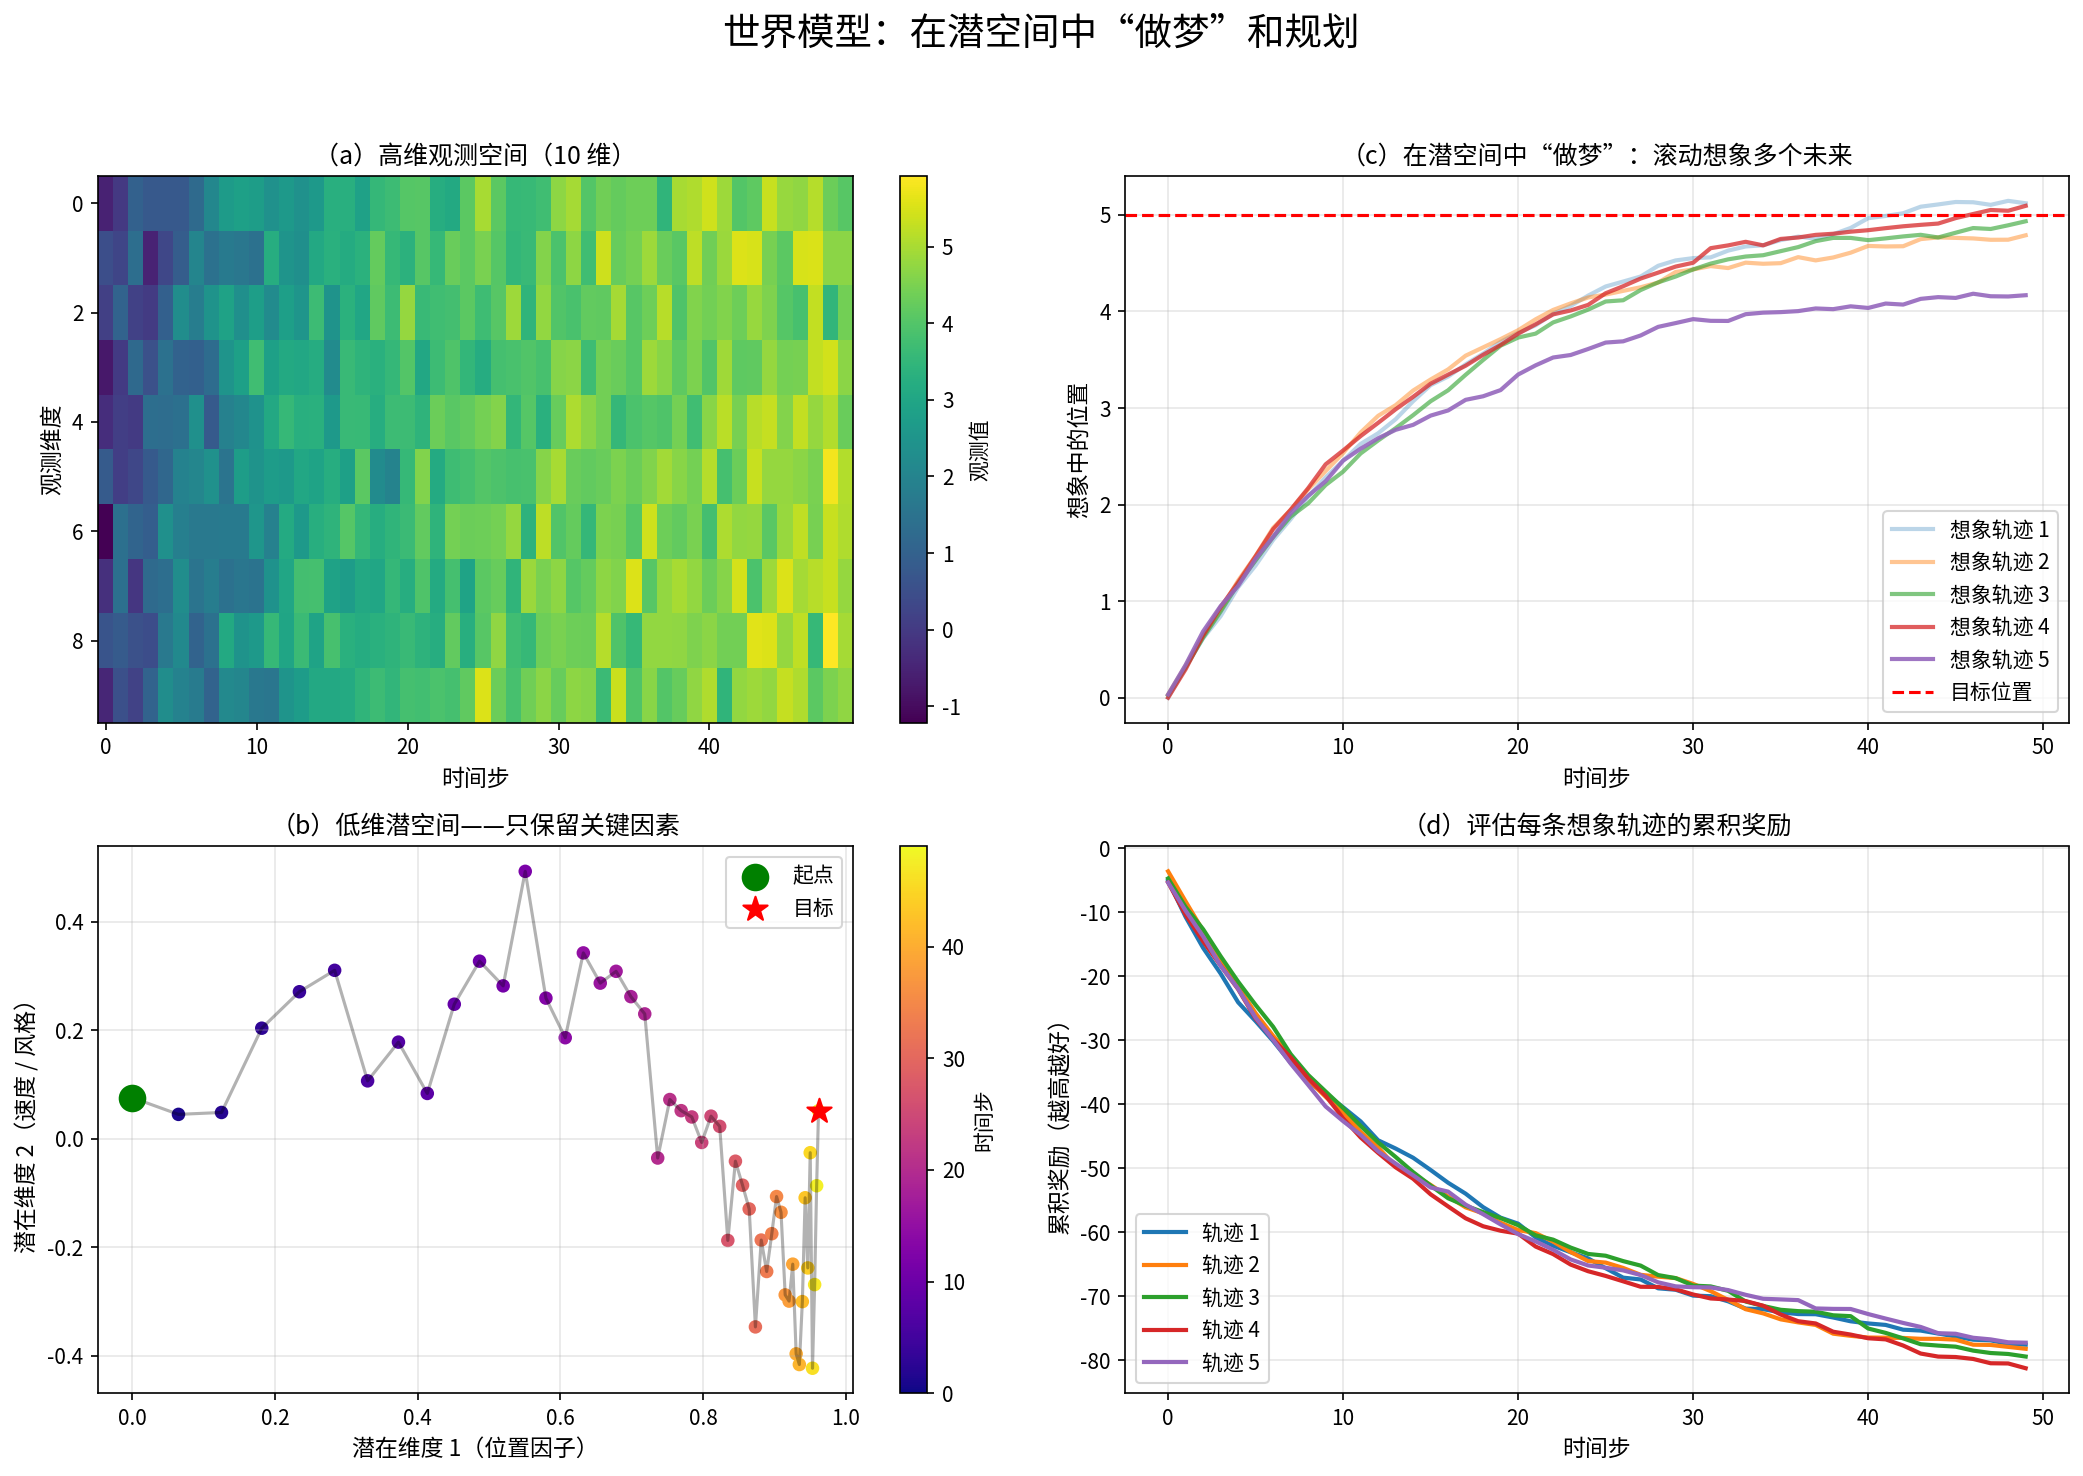
\includegraphics[width=0.95\textwidth]{figs_chap16/latent_dynamics.png}

\caption{潜空间动力学模型示意图。(a)高维观测数据难以直接处理；(b)编码器将其压缩到2维潜空间，清晰显示状态演化；(c)在潜空间中可以"做梦"——想象多条可能的未来轨迹；(d)评估每条轨迹的累积奖励，选择最优动作。}

\label{fig:latent_dynamics}

\end{figure}

 

\begin{example}[Dreamer算法：在梦中学习]

\marginnote{Dreamer是DeepMind提出的世界模型强化学习方法。它的核心思想是：在潜空间中"做梦"，想象可能的未来，然后在想象中学习策略。}

 

Dreamer算法的工作流程就像人类做白日梦：

 

\textbf{第一步：学习世界模型}

\begin{itemize}

    \item 收集真实环境中的经验$(o_1, a_1, r_1, o_2, \ldots)$

    \item 训练编码器、动力学模型、解码器

\end{itemize}

 

\textbf{第二步：在想象中规划}

\begin{itemize}

    \item 从当前潜态$z_t$出发

    \item 在潜空间中"展开"未来：$z_{t+1} = f(z_t, a_t)$

    \item 预测每一步的奖励：$\hat{r}_t = R(z_t)$

    \item 尝试不同的动作序列，找到累积奖励最高的那个

\end{itemize}

 

\textbf{第三步：执行并学习}

\begin{itemize}

    \item 执行规划得到的动作

    \item 用新数据更新世界模型

\end{itemize}

 

这就像你在脑中"预演"打台球——你想象不同的击球方式，预测结果，选择最好的那个，然后才真正动手。

\end{example}

 

\begin{physicalintuition}

\textbf{潜空间与广义坐标的深刻联系}

 

回想拉格朗日力学：我们用\textbf{广义坐标}$q$来描述系统状态，而不是用笛卡尔坐标。广义坐标的选择应该"尊重约束"——比如用角度$\theta$描述单摆，而不是用$(x, y)$坐标。

 

潜空间就是神经网络学到的"广义坐标"！它应该：

\begin{itemize}

    \item 捕捉系统的本质自由度（单摆只有1个自由度）

    \item 忽略无关的细节（如光照变化、背景噪声）

    \item 使动力学方程尽可能简单

\end{itemize}

 

\textbf{好的潜空间 = 好的广义坐标 = 对称性和约束的正确表达}

\end{physicalintuition}

 

下面是潜空间动力学模型的伪代码，帮助理解其核心结构：

 

\begin{algorithm}[H]
\caption{潜空间世界模型的核心流程}
\begin{algorithmic}[1]
\Require 观测序列 $\{o_1, o_2, \ldots, o_T\}$，动作序列 $\{a_1, a_2, \ldots, a_{T-1}\}$
\State \textbf{// 第一步：编码——将高维观测压缩到低维潜空间}
\For{$t = 1$ to $T$}
    \State $z_t \gets \text{Encoder}(o_t)$ \Comment{例如：$256\times256$图像 $\to$ 64维向量}
\EndFor
\State \textbf{// 第二步：学习动力学——潜态如何随动作演化}
\For{$t = 1$ to $T-1$}
    \State $\hat{z}_{t+1} \gets \text{Dynamics}(z_t, a_t)$ \Comment{预测下一个潜态}
    \State $\text{loss} \gets \text{loss} + \|z_{t+1} - \hat{z}_{t+1}\|^2$ \Comment{预测误差}
\EndFor
\State \textbf{// 第三步：想象未来——在潜空间中"做梦"}
\State $z_{\text{current}} \gets \text{Encoder}(o_{\text{current}})$
\For{每个候选动作序列 $\{a_1, a_2, \ldots, a_H\}$}
    \State $z \gets z_{\text{current}}$
    \State $\text{total\_reward} \gets 0$
    \For{$h = 1$ to $H$}
        \State $z \gets \text{Dynamics}(z, a_h)$
        \State $\text{total\_reward} \gets \text{total\_reward} + \text{RewardPredictor}(z)$
    \EndFor
    \State 记录该动作序列的总奖励
\EndFor
\State \textbf{return} 总奖励最高的动作序列的第一个动作
\end{algorithmic}
\end{algorithm}

 

% ====================================================================================

\section{具身智能的数学本质：安全约束下的控制}

% ====================================================================================

 

世界模型告诉我们"世界会怎么变"。但对于\textbf{具身智能}（Embodied Intelligence）——机器人、自动驾驶、无人机——光有预测还不够。

 

我们还需要回答：\textbf{如何在物理约束下安全地行动？}

 

\subsection{约束的本质变了}

 

回顾我们在第一章学过的拉格朗日力学。当时的约束是这样的：

\begin{equation}
    \mathcal{L} = T - V + \lambda g(q)
\end{equation}

 

这里的约束$g(q) = 0$是\textbf{等式约束}——比如单摆必须沿圆弧运动，系统没有选择。

 

但在机器人控制中，约束变成了\textbf{不等式约束}——有一片"禁区"，系统不能进入：

\begin{itemize}

    \item \textbf{安全边界}：$\text{距离障碍物}(x) \geq d_{\min}$（不能撞墙）

    \item \textbf{关节限位}：$q_{\min} \leq q \leq q_{\max}$（机械臂不能弯曲超过极限）

    \item \textbf{摩擦锥}：$\|f_{\text{切向}}\| \leq \mu f_{\text{法向}}$（脚不能打滑）

    \item \textbf{能量约束}：$\|u\|^2 \leq u_{\max}^2$（电机功率有限）

\end{itemize}

 

\begin{example}[等式约束 vs 不等式约束]

\begin{itemize}

    \item \textbf{等式约束}：火车必须在轨道上（没得选）

    \item \textbf{不等式约束}：汽车不能开到悬崖下面（有一片禁区，但路很宽）

\end{itemize}

\end{example}

 

\subsection{控制障碍函数：安全的数学保证}

 

如何保证机器人"永远不会撞墙"？这听起来是一个很强的要求——我们需要一个数学工具来提供\textbf{安全保证}。

 

\begin{definition}[安全集合与障碍函数——用通俗语言解释]

想象你在一个房间里，房间中央有一根柱子（障碍物）。我们定义一个函数$h(x)$：

 

\begin{equation}
    h(x) = \text{（你离柱子的距离）} - \text{（安全距离）}
\end{equation}

 

这个函数告诉我们：

\begin{itemize}

    \item $h(x) > 0$：你离柱子足够远，\textbf{安全}

    \item $h(x) = 0$：你刚好在安全边界上，\textbf{临界}

    \item $h(x) < 0$：你离柱子太近了，\textbf{危险}！

\end{itemize}

 

\textbf{安全集合}就是所有$h(x) \geq 0$的点构成的区域。

\end{definition}

 

更具体地，对于一个位于$x_{\text{obs}}$的圆形障碍物，安全距离为$d$，障碍函数可以定义为：

\begin{equation}
    h(x) = \|x - x_{\text{obs}}\|^2 - d^2
\end{equation}

 

这里$\|x - x_{\text{obs}}\|$是你到障碍物中心的距离。

 

\begin{theorem}[控制障碍函数条件——如何保证安全？]

\label{thm:cbf}

考虑一个受控系统：

\begin{equation}
    \dot{x} = f(x) + g(x)u
\end{equation}

其中$x$是状态，$u$是控制输入，$f(x)$是系统的自然演化，$g(x)$描述控制如何影响系统。

 

\textbf{关键问题}：我们想让$h(x)$永远保持非负（永远安全）。根据微积分，$h$的变化率是：

\begin{equation}
    \dot{h} = \frac{\partial h}{\partial x} \cdot \dot{x} = \frac{\partial h}{\partial x} \cdot (f(x) + g(x)u)
\end{equation}

 

\textbf{核心条件}：如果我们能保证

\begin{equation}
    \boxed{\dot{h}(x, u) \geq -\alpha \cdot h(x)}
\end{equation}

其中$\alpha > 0$是一个正常数，那么安全集合$h(x) \geq 0$是\textbf{前向不变}的——一旦进入安全区域，永远不会离开。

\end{theorem}

 

\begin{physicalintuition}

\textbf{为什么这个条件能保证安全？}

 

条件$\dot{h} \geq -\alpha h$的含义是：

\begin{itemize}

    \item 当$h$很大时（离危险很远），$\dot{h}$可以是负的——允许靠近

    \item 当$h$接近0时（快到边界了），$\dot{h}$必须接近0或为正——不能再靠近

    \item 当$h = 0$时（恰好在边界上），$\dot{h} \geq 0$——只能离开，不能进入危险区

\end{itemize}

 

这就像一个"软弹簧"把你推离危险区域——越靠近边界，推力越大。

\end{physicalintuition}

 

\begin{keyformula}[title=基于CBF的安全控制器]

假设我们有一个\textbf{标称控制器}$u_{\text{ref}}(x)$——这是我们"想要"的控制（比如"直线走向目标"）。

 

问题是：$u_{\text{ref}}$可能会导致碰撞。我们需要找一个\textbf{尽量接近}$u_{\text{ref}}$但\textbf{保证安全}的控制$u^*$。

 

这是一个\textbf{二次规划}（QP）问题：

\begin{equation}
    u^*(x) = \arg\min_{u} \frac{1}{2}\|u - u_{\text{ref}}(x)\|^2
\end{equation}

\begin{equation}
    \text{约束条件：} \quad \underbrace{\frac{\partial h}{\partial x}f(x)}_{\text{自然漂移}} + \underbrace{\frac{\partial h}{\partial x}g(x) \cdot u}_{\text{控制效果}} + \alpha h(x) \geq 0
\end{equation}

 

\textbf{直观解释}：在所有满足安全约束的控制中，选择和原计划最接近的那个。

\end{keyformula}

 

好消息是，这个QP有\textbf{闭式解}！利用拉格朗日乘子法（KKT条件）：

\begin{equation}
    u^* = u_{\text{ref}} - \lambda^* \left(\frac{\partial h}{\partial x}g(x)\right)^T
\end{equation}

其中$\lambda^* \geq 0$是拉格朗日乘子，只在约束激活（接近危险）时非零。

 

\begin{physicalintuition}

\textbf{CBF与拉格朗日力学的深刻联系}

 

这里的$\lambda^*$和拉格朗日力学中的约束力$\lambda$有着相同的物理意义！

 

\textbf{拉格朗日力学}：

\begin{itemize}

    \item 约束力$\lambda$维持等式约束$g(q) = 0$

    \item $\lambda$垂直于约束面，阻止系统"穿出"

\end{itemize}

 

\textbf{CBF控制}：

\begin{itemize}

    \item 安全修正项$\lambda^* (\nabla h \cdot g)^T$维持不等式约束$h(x) \geq 0$

    \item $\lambda^*$只在接近边界时激活，产生"斥力"

\end{itemize}

 

\textbf{统一视角}：两者都是\textbf{约束优化}——拉格朗日乘子是"违反约束的代价"。

\end{physicalintuition}

 

\subsection{实验结果：CBF控制器的效果}

 

下面我们通过一个简单的实验来展示CBF控制器的效果。场景设置：

\begin{itemize}

    \item 起点：$(0, 0)$

    \item 目标：$(10, 10)$

    \item 障碍物：位于$(5, 5)$，安全距离$d = 1.5$

    \item 标称控制器：直接朝目标方向走

\end{itemize}

 

\begin{figure}[htbp]

\centering

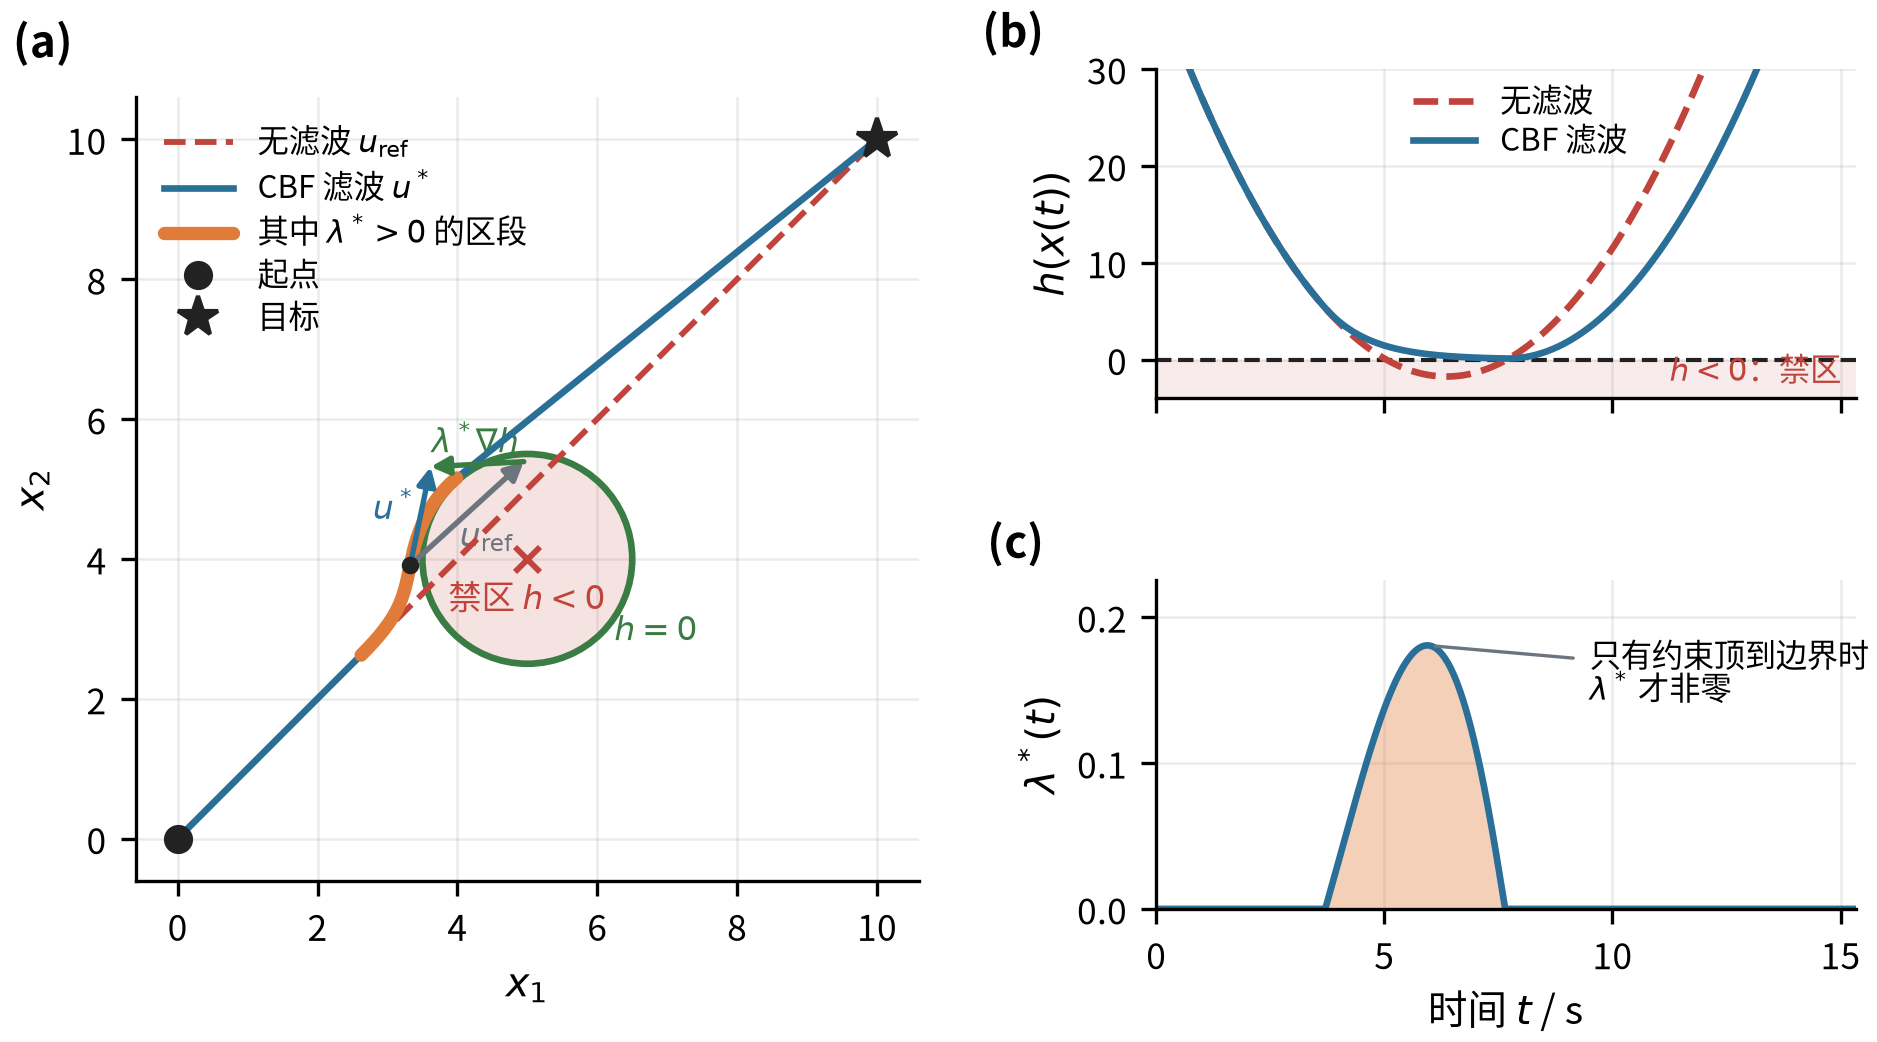
\includegraphics[width=0.95\textwidth]{figs_chap16/cbf_controller.png}

\caption{CBF安全控制器实验结果。(a)无CBF时，智能体直线冲向目标，穿过障碍物！(b)有CBF时，智能体绕开障碍物安全到达目标。(c)障碍函数$h(x)$随时间变化：无CBF时$h$变负（进入危险区），有CBF时$h$始终非负。(d)控制输入对比：CBF只在必要时（接近障碍物时）修正控制。}

\label{fig:cbf_controller}

\end{figure}

 

\textbf{关键观察}：

\begin{enumerate}

    \item \textbf{安全保证}：有CBF时，障碍函数$h(x)$始终保持非负，系统永远不会进入危险区域。

    \item \textbf{最小干预}：CBF控制器是"懒惰"的——只有当系统接近危险边界时才会干预。在远离障碍物的地方，$u_{\text{safe}} \approx u_{\text{ref}}$。

    \item \textbf{光滑绕行}：系统自然地绕开障碍物，轨迹平滑，没有突变。

\end{enumerate}

 

\begin{figure}[htbp]

\centering

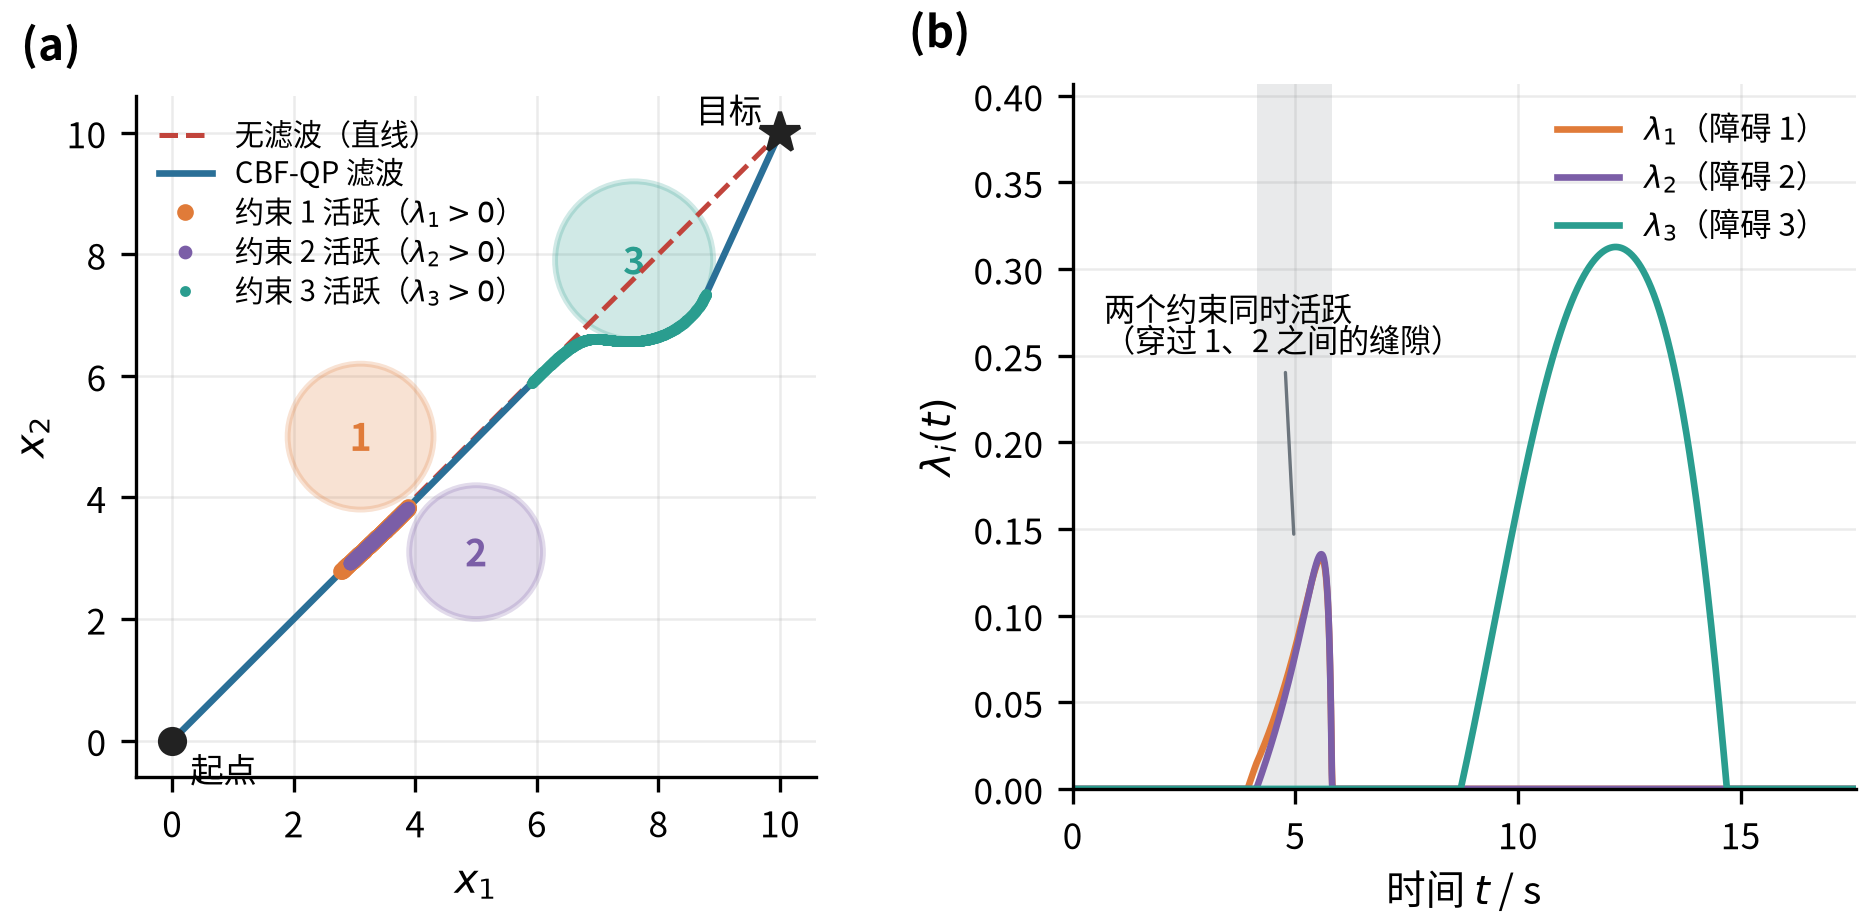
\includegraphics[width=0.75\textwidth]{figs_chap16/multi_obstacle.png}

\caption{多障碍物环境下的CBF避障。智能体从起点出发，自动规划路径绕过所有障碍物到达目标。颜色深浅表示时间推进。}

\label{fig:multi_obstacle}

\end{figure}

 

CBF方法可以自然地扩展到\textbf{多障碍物}场景：对每个障碍物定义一个障碍函数$h_i(x)$，然后在控制器中同时满足所有约束。

 

\begin{algorithm}[H]
\caption{CBF安全控制器伪代码}
\begin{algorithmic}[1]
\Require 当前位置 $x$，目标位置 $x_{\text{goal}}$，障碍物位置 $x_{\text{obs}}$，安全距离 $d$
\State \textbf{// 第一步：计算标称控制（朝目标走）}
\State $u_{\text{ref}} \gets \text{方向}(x_{\text{goal}} - x) \times \text{速度}$
\State \textbf{// 第二步：计算障碍函数及其梯度}
\State $h \gets \|x - x_{\text{obs}}\|^2 - d^2$ \Comment{正表示安全，负表示危险}
\State $\nabla h \gets 2(x - x_{\text{obs}})$ \Comment{指向远离障碍物的方向}
\State \textbf{// 第三步：检查安全约束}
\If{$\nabla h \cdot u_{\text{ref}} + \alpha \cdot h \geq 0$}
    \State \textbf{return} $u_{\text{ref}}$ \Comment{标称控制已经安全，无需修正}
\EndIf
\State \textbf{// 第四步：计算安全修正}
\State $\lambda \gets -\frac{\nabla h \cdot u_{\text{ref}} + \alpha \cdot h}{\|\nabla h\|^2}$
\State $u_{\text{safe}} \gets u_{\text{ref}} - \lambda \cdot \nabla h$ \Comment{沿梯度方向修正}
\State \textbf{return} $u_{\text{safe}}$
\end{algorithmic}
\end{algorithm}

 

% ====================================================================================

\section{可微物理：当牛顿定律变成计算图}

% ====================================================================================

 

\subsection{从黑盒到白盒}

 

传统的物理仿真器（如游戏引擎）是\textbf{黑盒}：你输入状态和控制，它输出下一个状态，但你无法知道"输出对输入的导数是多少"。

 

\textbf{可微物理}（Differentiable Physics）的思想是：把物理定律写成\textbf{可自动微分}的计算图。

 

\begin{definition}[可微物理仿真器]

可微物理仿真器将物理仿真实现为：

\begin{equation}
    x_{t+1} = \text{PhysicsStep}(x_t, u_t; \theta)
\end{equation}

其中$\theta$是物理参数（质量、刚度、摩擦系数等），整个函数对$(x_t, u_t, \theta)$都是\textbf{可微的}——可以计算梯度！

\end{definition}

 

\begin{example}[为什么需要可微？]

想象你在训练一个机器人走路：

\begin{itemize}

    \item 你有一个策略网络$\pi_\theta$，输出每个关节的力矩

    \item 物理仿真器计算机器人的运动

    \item 你想最小化"摔倒次数"

\end{itemize}

 

\textbf{传统方法}（强化学习）：随机尝试，看哪个好，很慢。

 

\textbf{可微物理}：直接计算"如果我改变策略参数，摔倒次数会怎么变"——梯度下降，很快。

\end{example}

 

\begin{advantage}[可微物理的三大优势]

\textbf{1. 策略优化}——直接优化策略参数：

\begin{equation}
    \theta^* = \arg\min_\theta \mathcal{L}(\text{Simulate}(\pi_\theta))
\end{equation}

用梯度下降代替随机搜索！

 

\textbf{2. 系统辨识}——从观测数据学习物理参数：

\begin{equation}
    \phi^* = \arg\min_\phi \|x_{\text{真实}} - x_{\text{仿真}}(\phi)\|^2
\end{equation}

给定轨迹数据，反推质量、摩擦系数等。

 

\textbf{3. Sim-to-Real迁移}——同时优化策略和物理参数，缩小仿真与现实的差距。

\end{advantage}

 

\subsection{实验：弹簧-质点系统的可微仿真}

 

让我们用一个简单的例子来说明可微物理的威力：\textbf{弹簧-质点系统}。

 

物理方程：

\begin{equation}
    m\ddot{x} = -kx - c\dot{x} + u
\end{equation}

其中：

\begin{itemize}

    \item $m$：质量

    \item $k$：弹簧刚度

    \item $c$：阻尼系数

    \item $u$：外力（控制输入）

\end{itemize}

 

\begin{figure}[htbp]

\centering

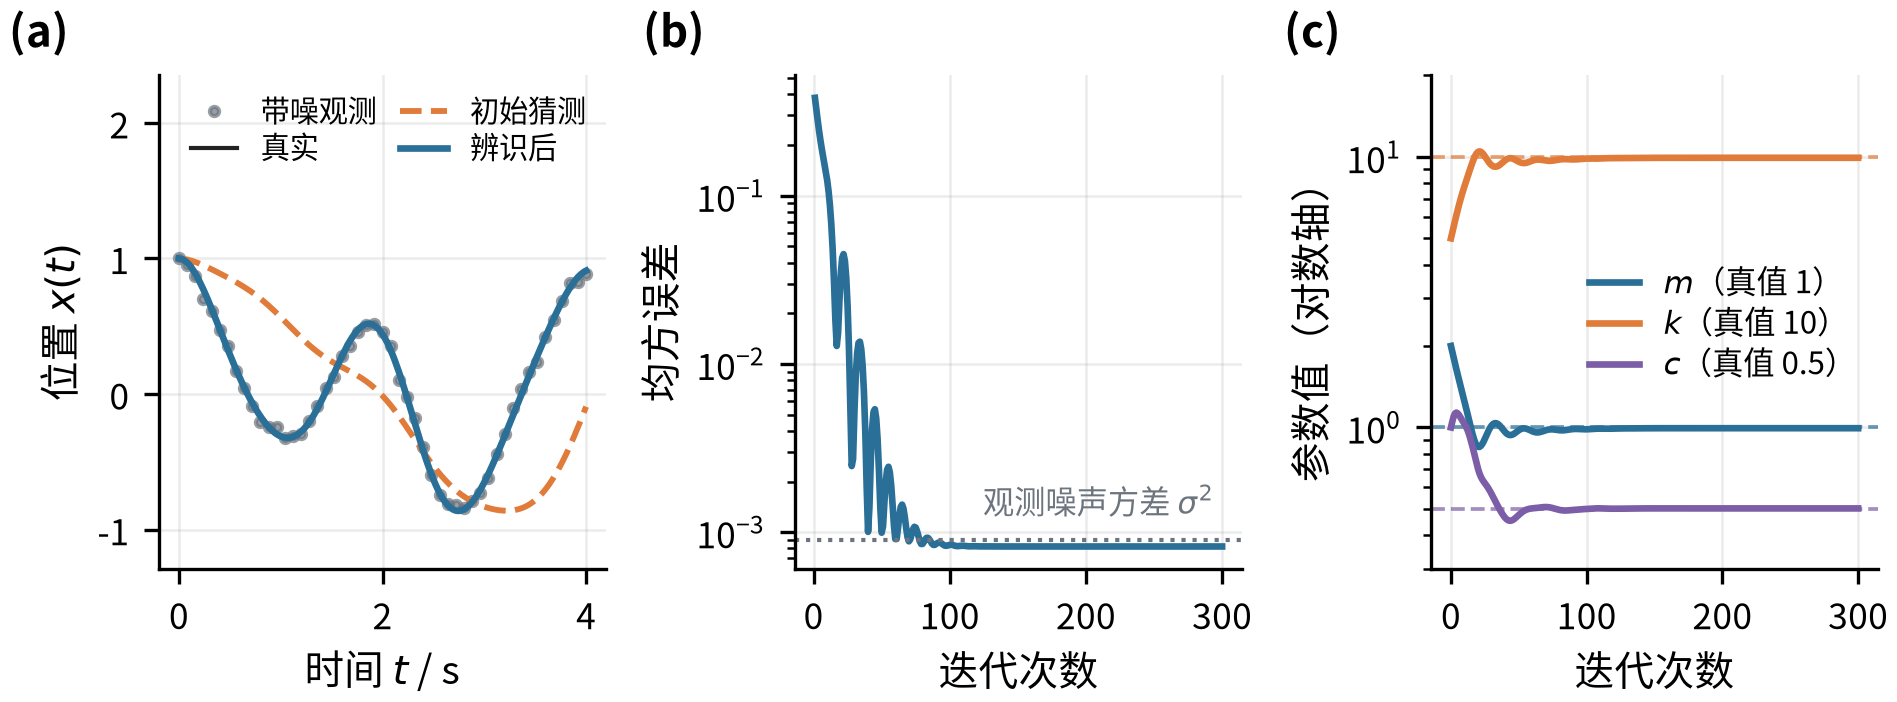
\includegraphics[width=0.95\textwidth]{figs_chap16/differentiable_physics.png}

\caption{可微物理系统辨识实验。(a)弹簧-质点系统的真实轨迹（$m=1, k=10, c=0.5$）；(b)损失函数随迭代下降；(c)三个物理参数逐渐收敛到真值；(d)学习到的模型能准确预测轨迹。}

\label{fig:differentiable_physics}

\end{figure}

 

\textbf{实验设置}：

\begin{itemize}

    \item 真实参数：$m=1, k=10, c=0.5$

    \item 初始猜测：$m=2, k=5, c=1$（故意猜错）

    \item 目标：从带噪声的观测数据中恢复真实参数

\end{itemize}

 

\textbf{实验结果分析}：

\begin{enumerate}

    \item \textbf{损失下降}：均方误差从初始值迅速下降两个数量级

    \item \textbf{参数收敛}：经过100次迭代，三个参数都接近真值

    \item \textbf{模型准确}：学到的模型（红色虚线）与真实轨迹（蓝色实线）高度吻合

\end{enumerate}

 

这个实验展示了可微物理的核心能力：\textbf{从数据中学习物理参数}。在更复杂的场景中（如机器人、流体），同样的方法可以用来校准仿真器，使其更接近真实世界。

 

\subsection{相空间：理解动力系统的窗口}

 

\begin{definition}[相空间——另一种看世界的方式]

对于一个力学系统，\textbf{相空间}是由位置$x$和速度$v$组成的空间。系统的状态是相空间中的一个点，随时间演化形成一条\textbf{轨迹}。

\end{definition}

 

\begin{figure}[htbp]

\centering

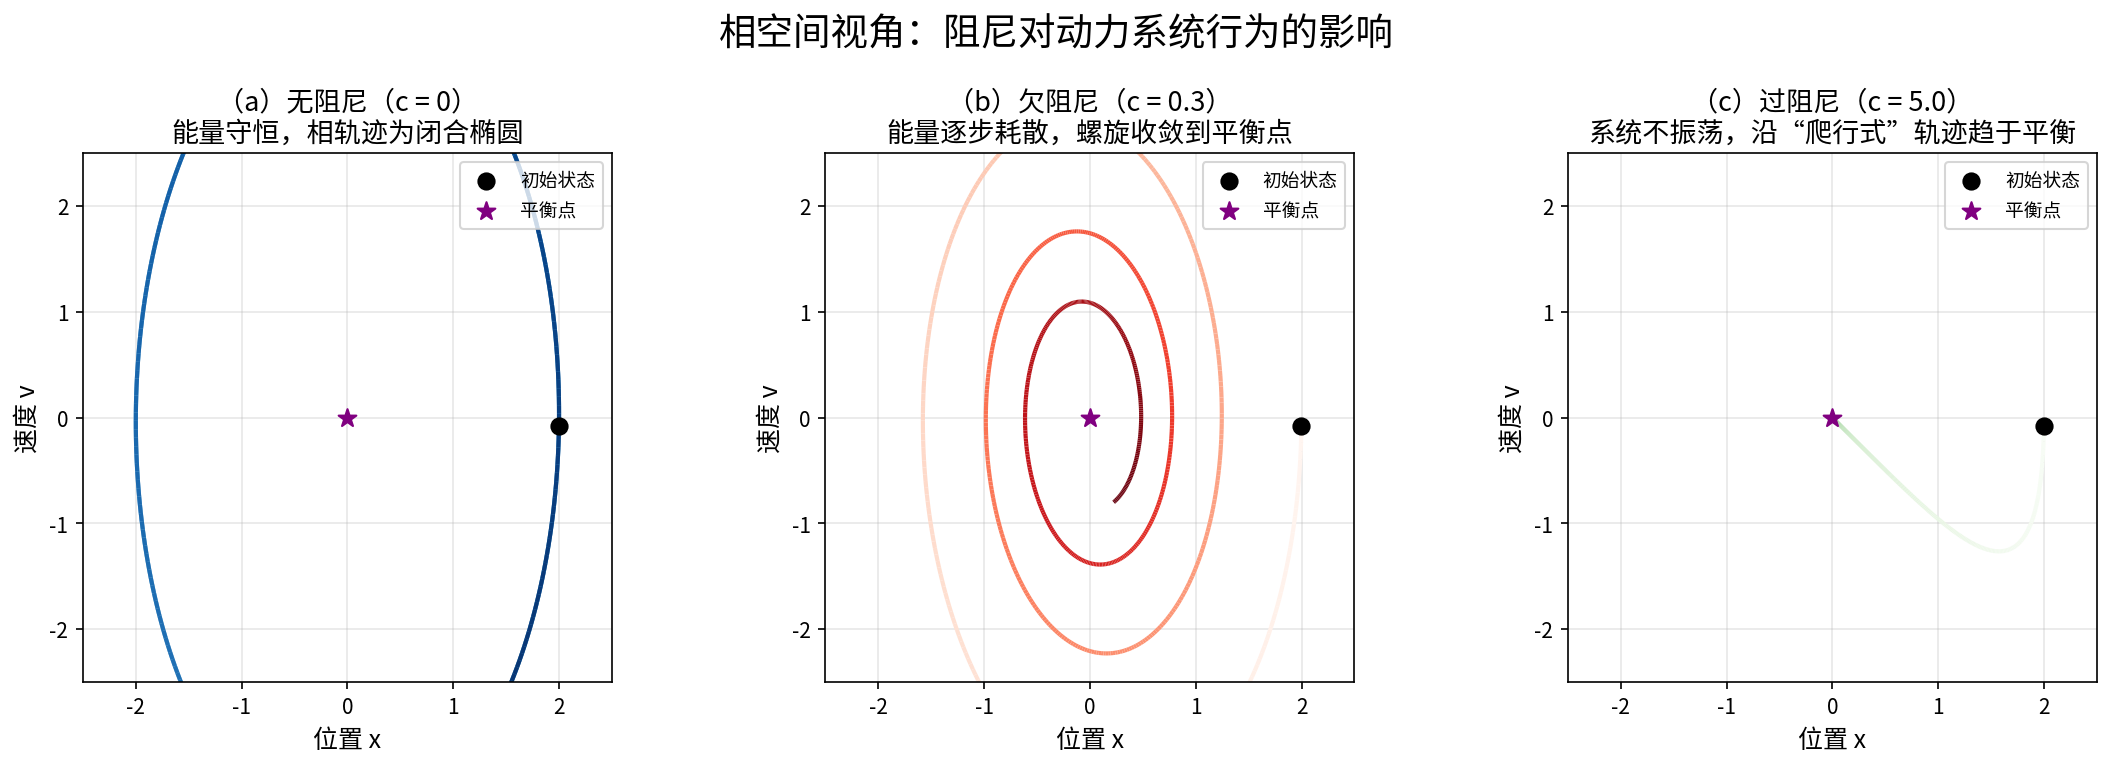
\includegraphics[width=0.95\textwidth]{figs_chap16/phase_space.png}

\caption{弹簧-质点系统的相空间轨迹。(a)无阻尼：能量守恒，轨迹是闭合的椭圆；(b)欠阻尼：能量逐渐耗散，轨迹螺旋趋向平衡点；(c)过阻尼：系统"懒洋洋"地直接趋向平衡点。}

\label{fig:phase_space}

\end{figure}

 

\textbf{相空间的物理意义}：

\begin{itemize}

    \item \textbf{无阻尼}（$c=0$）：总能量$E = \frac{1}{2}mv^2 + \frac{1}{2}kx^2$守恒，轨迹是椭圆

    \item \textbf{欠阻尼}（$c$较小）：能量逐渐耗散，轨迹螺旋向内

    \item \textbf{过阻尼}（$c$较大）：系统被"拖住"，缓慢趋向平衡

\end{itemize}

 

相空间是理解动力系统的重要工具——它让我们"一眼看出"系统的长期行为。

 

% ====================================================================================

\section{终极猜想：自由能原理与智能的统一理论}

% ====================================================================================

 

\marginnote{\textbf{Karl Friston}(1959--)：英国神经科学家，伦敦大学学院教授，英国皇家学会院士。他是世界上被引用最多的神经科学家，h-index超过250。他发明了脑成像分析的标准工具SPM，2000年代后致力于自由能原理，试图用单一数学框架统一大脑的感知、学习、决策。}

 

在本章的最后，让我们探讨一个大胆的问题：\textbf{智能的本质是什么？}

 

\subsection{惊奇最小化：一个统一的原理}

 

Karl Friston提出的\textbf{自由能原理}（Free Energy Principle）给出了一个优雅的答案：

 

\begin{philosophy}

\textbf{核心观点}：生命体（智能体）存在的目的，就是\textbf{最小化变分自由能}。

 

用更直白的话说：智能体试图\textbf{最小化惊奇}（Surprise）——让世界的行为符合自己的预期。

\end{philosophy}

 

\begin{example}[什么是"惊奇"？]

\begin{itemize}

    \item 你预期太阳从东边升起——太阳真的从东边升起——\textbf{不惊奇}

    \item 你预期房间里有椅子——椅子还在——\textbf{不惊奇}

    \item 你预期咖啡是热的——喝了一口是冰的——\textbf{惊奇！}

\end{itemize}

 

"惊奇"的数学定义是：$\text{惊奇} = -\log P(\text{观测})$

 

观测越不可能（越意外），惊奇越大。

\end{example}

 

\begin{definition}[变分自由能——稍微技术一点]

给定观测$o$和内部状态$s$（智能体的"信念"），\textbf{变分自由能}定义为：

\begin{equation}
    F = \E_{q(s)}[\log q(s) - \log p(s, o)]
\end{equation}

这可以分解为两部分：

\begin{equation}
    F = \underbrace{\text{KL}(q(s) \| p(s|o))}_{\text{信念与真实的差距}} + \underbrace{(-\log p(o))}_{\text{惊奇}}
\end{equation}

\end{definition}

 

\subsection{感知与行动的统一}

 

自由能原理最优美的地方在于：它用\textbf{同一个目标函数}统一了\textbf{感知}和\textbf{行动}。

 

\begin{figure}[htbp]

\centering

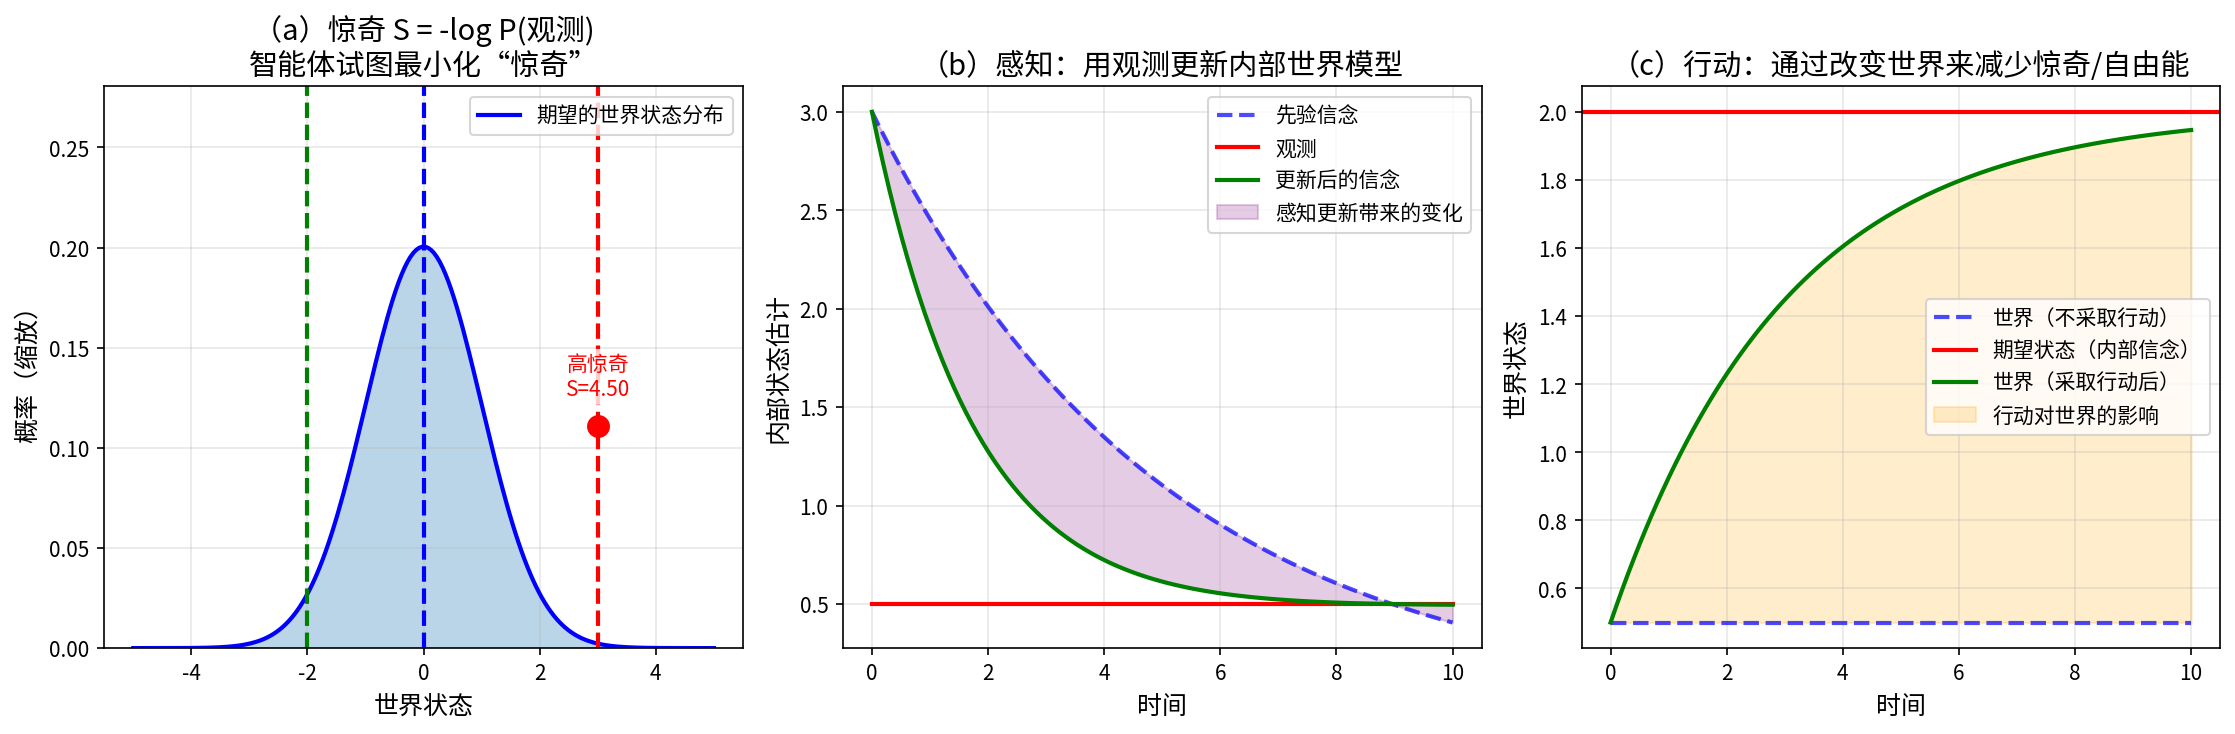
\includegraphics[width=0.95\textwidth]{figs_chap16/free_energy.png}

\caption{自由能原理示意图。(a)惊奇的定义：观测越偏离预期，惊奇越大；(b)感知：更新信念使之匹配观测；(c)行动：改变世界使之匹配信念。两者都在最小化惊奇！}

\label{fig:free_energy}

\end{figure}

 

\begin{keyformula}[title=感知与行动的统一]

\textbf{感知}（Perception）：更新内部信念$s$以最小化自由能

\begin{equation}
    s^* = \arg\min_s F(s, o) \quad \text{（"我看到了什么？更新我的信念"）}
\end{equation}

 

\textbf{行动}（Action）：改变世界状态以最小化\textbf{期望}自由能

\begin{equation}
    a^* = \arg\min_a \E_{p(o|a)}[F(s, o)] \quad \text{（"世界不符合预期？改变它！"）}
\end{equation}

 

两者都是在最小化"惊奇"——感知通过改变信念，行动通过改变世界！

\end{keyformula}

 

\begin{example}[为什么人在黑暗中感到不安？]

用自由能原理解释：

\begin{itemize}

    \item 在黑暗中，视觉输入的不确定性很高

    \item 高不确定性 = 难以预测 = 高惊奇

    \item 智能体天生"不喜欢"惊奇

    \item 所以人会感到不安，并采取行动（开灯、走到明亮处）来减少不确定性

\end{itemize}

\end{example}

 


 

% ====================================================================================

\section{习题}

% ====================================================================================

 

\subsection{概念题}

 

\begin{exercise}[世界模型的范式比较]

比较生成式世界模型和JEPA两种范式：

\begin{enumerate}

    \item 用自己的话解释：为什么LeCun认为"预测像素是浪费算力"？

    \item 从"约束优化"的角度，两者的目标函数有什么不同？

    \item 举一个生活中的例子，说明"学习本质"比"记忆细节"更重要。

\end{enumerate}

\end{exercise}

 

\begin{exercise}[CBF的物理意义]

考虑一个机器人在房间里移动，房间中央有一根柱子。

\begin{enumerate}

    \item 写出障碍函数$h(x)$的表达式（设机器人位置为$x$，柱子位置为$x_c$，安全距离为$r$）。

    \item 解释：为什么条件$\dot{h} \geq -\alpha h$能保证安全？

    \item CBF中的$\lambda^*$和拉格朗日力学中的约束力$\lambda$有什么相似之处？

\end{enumerate}

\end{exercise}

 

\begin{exercise}[自由能原理]

用自由能原理解释以下现象：

\begin{enumerate}

    \item 为什么人在黑暗的房间里会感到不安？

    \item 为什么我们喜欢有规律、可预测的生活？

    \item "好奇心"如何用自由能原理解释？（提示：探索可以减少未来的不确定性）

\end{enumerate}

\end{exercise}

 

\subsection{计算题}

 

\begin{exercise}[简单的CBF计算]

设系统状态$x \in \R$，动力学为$\dot{x} = u$（控制直接决定速度），障碍函数$h(x) = x - 1$（不能进入$x < 1$的区域）。

\begin{enumerate}

    \item 写出CBF条件$\dot{h} \geq -\alpha h$的具体形式。

    \item 如果标称控制$u_{\text{ref}} = -1$（朝危险方向走），当$x = 2$时，CBF会如何修正？

    \item 当$x = 1.1$时呢？

\end{enumerate}

\end{exercise}

 

\begin{exercise}[相空间分析]

对于弹簧-质点系统$m\ddot{x} = -kx - c\dot{x}$：

\begin{enumerate}

    \item 写出相空间$(x, v)$中的动力学方程。

    \item 当$c = 0$时，证明能量$E = \frac{1}{2}mv^2 + \frac{1}{2}kx^2$守恒。

    \item 当$c > 0$时，证明$\frac{dE}{dt} \leq 0$（能量只能减少）。

\end{enumerate}

\end{exercise}

 

\subsection{思考题}

 

\begin{exercise}[开放讨论]

本章提出"智能 = 在约束下寻找最优"。你认为这个观点能解释人类智能吗？有什么局限性？

\end{exercise}

% ====================================================================================
\section*{本章结语：从牛顿到智能}
\addcontentsline{toc}{section}{本章结语}
% ====================================================================================

\vspace{0.5cm}

当牛顿在1687年写下$F = ma$时，他大概不会想到，这个简单的方程会成为理解智能的钥匙。

\vspace{0.3cm}

当拉格朗日在1788年用变分法重写力学时，他大概不会想到，他的$\lambda$乘子会在300年后被用来训练神经网络、控制机器人、理解大脑。

\vspace{0.3cm}

而今天，当我们站在人工智能革命的浪潮中，回望这本书走过的旅程：

\begin{itemize}
    \item 从\textbf{第一章}的KKT条件，到\textbf{第十章}的强化学习
    \item 从\textbf{有限元}的$KU=F$，到\textbf{PINN}的物理信息损失
    \item 从\textbf{单智能体}的最优控制，到\textbf{多智能体}的纳什均衡
    \item 从\textbf{经典力学}的约束力，到\textbf{世界模型}的潜空间动力学
\end{itemize}

我们发现，所有这些看似迥异的领域，竟然都在诉说同一个故事：

\begin{keyformula}[title=全书的核心信息]
\begin{center}
\Large
\textbf{智能 = 在约束下寻找最优}
\end{center}

\vspace{0.3cm}

无论是石头滚下山坡，还是AlphaGo落子博弈；无论是单摆的简谐振动，还是GPT生成流畅的文字——它们都在做同一件事：在各自的约束条件下，寻找某种意义上的"最优解"。

\vspace{0.3cm}

\textbf{约束}定义了可能性的边界，\textbf{优化}选择了边界内的最佳路径。

\textbf{$\lambda$}不只是数学技巧，它是约束的"价格"，是物理的"力"，是信息的"代价"。
\end{keyformula}

\vspace{0.5cm}

\begin{philosophy}
\textbf{给读者的临别赠言}

\vspace{0.3cm}

如果你是大二的学生，正站在科学与工程的分岔路口，希望这本书能给你一个统一的视角：不要把物理、数学、计算机看成孤立的学科，它们是同一座大厦的不同房间。

\vspace{0.3cm}

当你下次遇到一个复杂问题时，不妨问自己三个问题：

\begin{enumerate}
    \item \textbf{目标是什么？}——我想最大化/最小化什么？
    \item \textbf{约束是什么？}——什么条件必须满足？
    \item \textbf{$\lambda$代表什么？}——约束的代价/价格/力是什么？
\end{enumerate}

这三个问题，能帮你把任何复杂问题，翻译成你已经熟悉的数学语言。
\end{philosophy}

\vspace{0.8cm}

\begin{center}
\Large
\textit{愿你在约束中找到自由，在优化中发现智慧。}

\vspace{0.5cm}

\normalsize
\textbf{全书完}
\end{center} 